\documentclass[final]{beamer}
\usepackage[scale=1.24]{beamerposter}
\usepackage{graphicx}			% allows us to import images
\usepackage{amsmath}
\usepackage{amssymb}   
\usepackage{graphicx}

\newcommand{\bb}[1]{\textbf{#1}}

%-----------------------------------------------------------
% Define the column width and poster size
% To set effective sepwid, onecolwid and twocolwid values, first choose how many columns you want and how much separation you want between columns
% The separation I chose is 0.024 and I want 4 columns
% Then set onecolwid to be (1-(4+1)*0.024)/4 = 0.22
% Set twocolwid to be 2*onecolwid + sepwid = 0.464
%-----------------------------------------------------------

\newlength{\sepwid}
\newlength{\onecolwid}
\newlength{\twocolwid}
\newlength{\threecolwid}
\setlength{\paperwidth}{48in}
\setlength{\paperheight}{36in}
\setlength{\sepwid}{0.024\paperwidth}
\setlength{\onecolwid}{0.22\paperwidth}
\setlength{\twocolwid}{0.464\paperwidth}
\setlength{\threecolwid}{0.708\paperwidth}
\setlength{\topmargin}{-0.5in}
\usetheme{confposter}
\usepackage{exscale}



%-----------------------------------------------------------
% The next part fixes a problem with figure numbering. Thanks Nishan!
% When including a figure in your poster, be sure that the commands are typed in the following order:
% \begin{figure}
% \includegraphics[...]{...}
% \caption{...}
% \end{figure}
% That is, put the \caption after the \includegraphics
%-----------------------------------------------------------

\usecaptiontemplate{
\small
\structure{\insertcaptionname~\insertcaptionnumber:}
\insertcaption}

%-----------------------------------------------------------
% Define colours (see beamerthemeconfposter.sty to change these colour definitions)
%-----------------------------------------------------------

\setbeamercolor{block title}{fg=ngreen,bg=white}
\setbeamercolor{block body}{fg=black,bg=white}
\setbeamercolor{block alerted title}{fg=white,bg=dblue!70}
\setbeamercolor{block alerted body}{fg=black,bg=dblue!10}

%-----------------------------------------------------------
% Name and authors of poster/paper/research
%-----------------------------------------------------------

\title{Criminal Pursuit on a Preferential Attachment Tree}
\author{Charlie Z. Marshak, M. Puck Rombach, Andrea L. Bertozzi, and Maria R. D'Orsogna}
\institute{Department of Mathematics and  Institute of Pure and Applied Mathematics \\at University of California, Los Angeles}

%-----------------------------------------------------------
% Start the poster itself
%-----------------------------------------------------------

\begin{document}
\begin{frame}[t]
\begin{columns}[t]												% the [t] option aligns the column's content at the top
\begin{column}{\sepwid}\end{column}			% empty spacer column


%-----------------------------------------------------------
%Begin COLUMN ONE
%-----------------------------------------------------------

\begin{column}{\onecolwid}


\begin{alertblock}{Part I: The Preferential Attachment Tree}
We model the growth of a criminal syndicate with a recursive preferential attachment tree, where preference is given to nodes closer to leaves or leaves themselves.  We represent the kingpin by a root node.
\end{alertblock}

 \begin{block}{The Growth Process}
Let $\bb T^0$ be a rooted seed tree and $\bb T^t$ be the tree at time $t$.   
 To obtain $\bb T^t$ from $\bb T^{t-1}$, we add $k$ new nodes to $\bb T^{t-1}$.  A leaf is a node without any children; these are the street criminals.  Let $d(j, t)$ denote the minimum distance from node $j$ to a leaf taken over all leaves in the tree.  Each new node 
 attaches to an existing node $j$ on $\bb T^{t-1}$ with probability proportional to weight $w(j, t-1)$.   The weight $w(j, t)$ of node $j$ at time $t$ is defined as:
\begin{align*}
w(j, t)  &:= \frac{1}{d(j, t)+1}
\end{align*}
\end{block}

\begin{block}{Node Density}
We found the node density depends on the distance to the root.  Figure [\ref{nd}] suggests a shifted gamma gamma ($\gamma$-)density approximates this relationship well.  The shifted $\gamma$-density is given by:
$$
\rho_{\alpha, \beta, s}(x) = \frac{\beta^\alpha}{\Gamma(\alpha)}(x - s)^{\alpha-1}e^{ -\beta (x-s)}.
$$
\begin{figure}
\includegraphics[width=0.8\linewidth]{nodedensity.pdf}
\caption{The number of nodes $N $ was $2,000; \; 4,000;\;6,000$ and the arrival rate was $k = 4$.  We averaged over 20 experiments.  $\bb T^0$ was a complete tertiary tree of height 3.  We fit the data with a shifted $\gamma$-density.}
\label{nd}
\end{figure}
\end{block}
\end{column}
%-----------------------------------------------------------
%END COLUMN ONE
%-----------------------------------------------------------


\begin{column}{\sepwid}\end{column}			% empty spacer column


%-----------------------------------------------------------
%BEGIN COLUMN TWO
%-----------------------------------------------------------

    

\begin{column}{\onecolwid}

\begin{block}{Degree Distribution}
A key feature of the Barab\'{a}si-Albert preferential attachment model [3] is its heavy-tailed degree distribution, which obeys a power-law.  From the data seen in Figure [\ref{DD}], we conjecture the degrees in this model are also heavy-tailed, and further, obeys an exponential law.
\begin{figure}
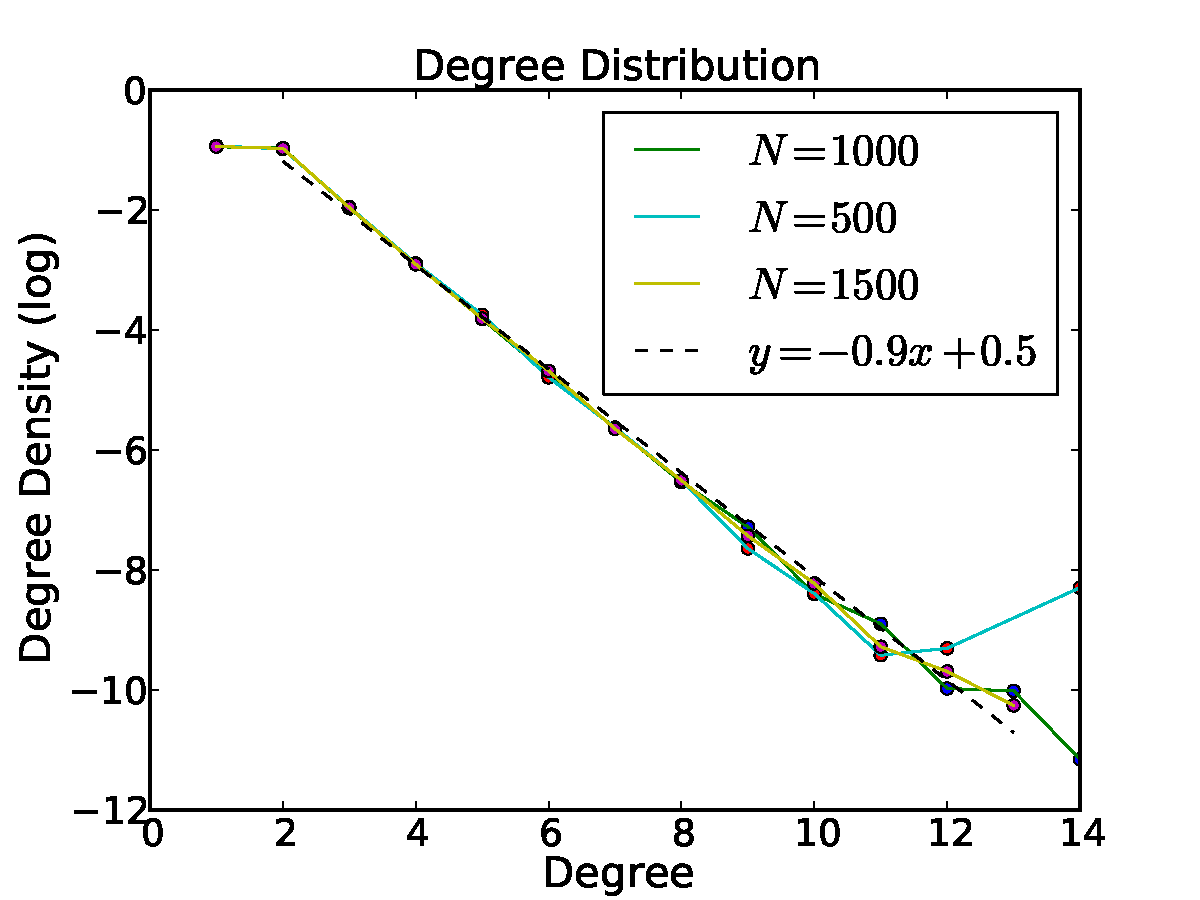
\includegraphics[width=0.65\linewidth]{DDPEAK.pdf}
\caption{The degree distribution appears to be exponentially distributed. }
\label{DD}
\end{figure}
\end{block}

 \begin{block}{Rate of Leaf Addition} 
 Leaves have the highest probability of recruitment and their distribution has important theoretical consequences.  
 %Also, this rate can be interpreted as the growth of ``street'' crime.  
 Figure [\ref{leaf}] suggests the rate of leaf addition is constant.
 \begin{figure}
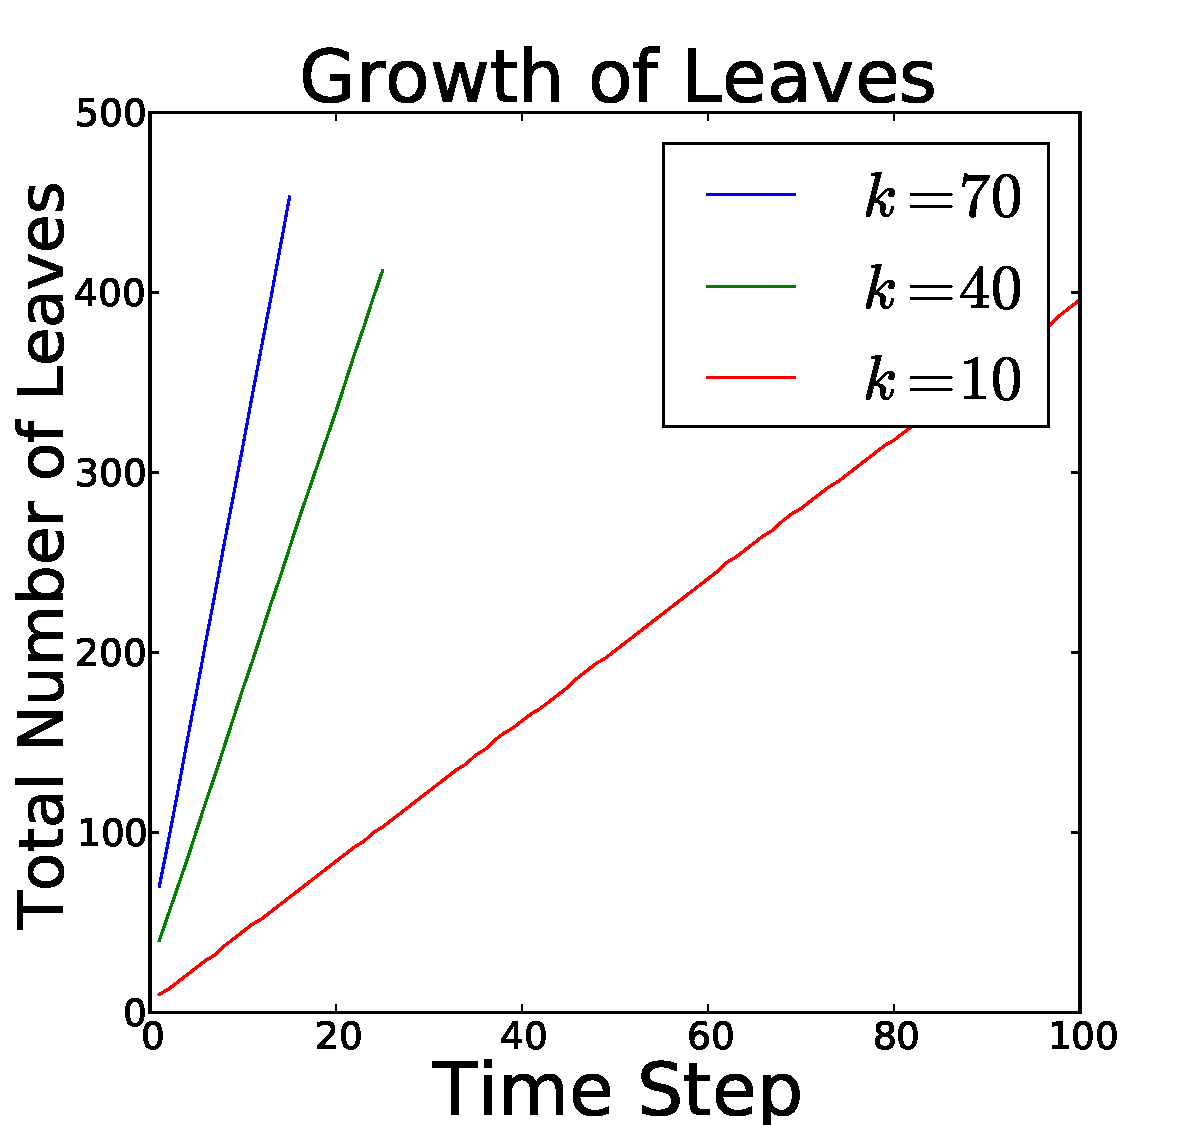
\includegraphics[width=0.45\linewidth]{leaves_per_timestep.pdf}
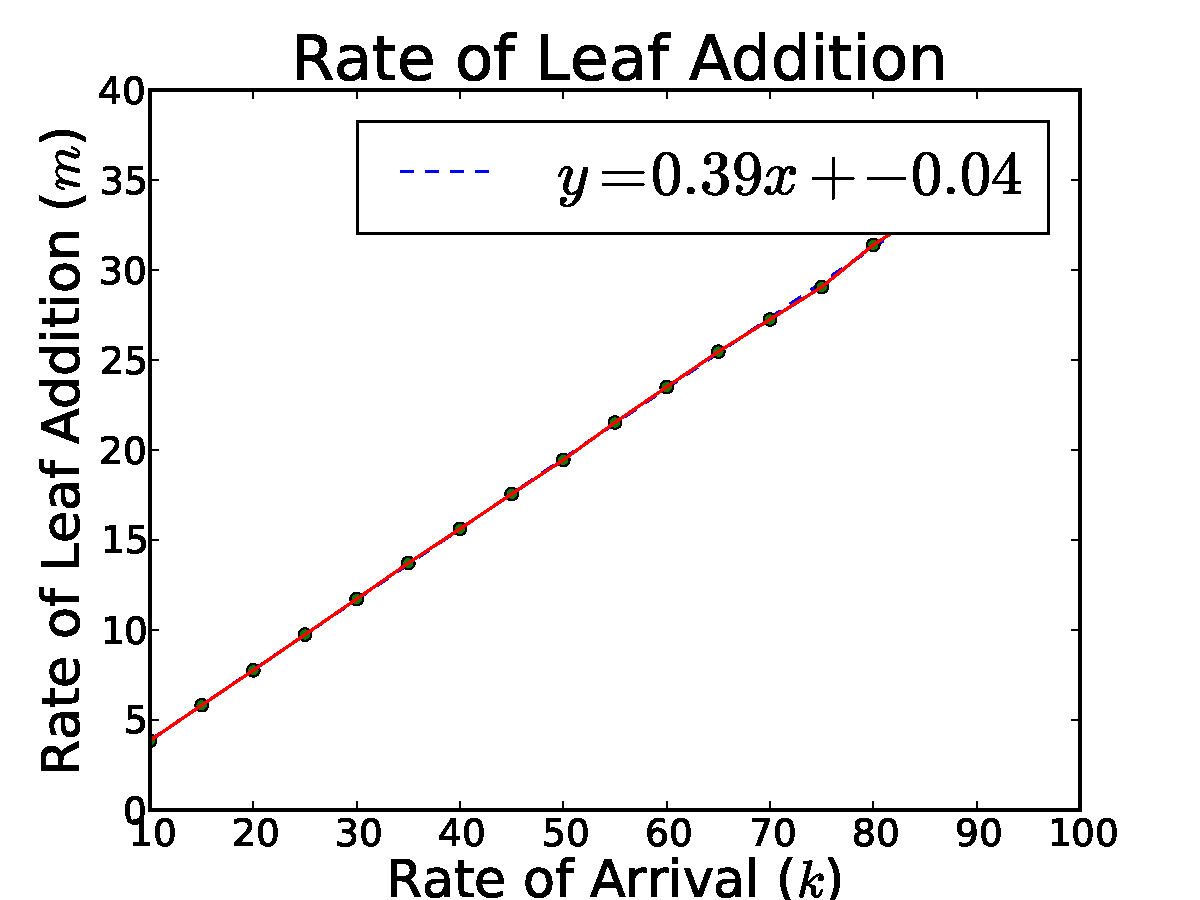
\includegraphics[width=0.5\linewidth, height = 4.5in]{slope_arrival.pdf}
\caption{$N = 1,000$ and $k$ is varied.  The relationship between number of leaves and time (left) appears linear; moreover, the slope of this relation appears to linearly depend on $k$ (right).}
\label{leaf}
\end{figure}
\end{block}




\begin{block}{Conjectures on Growth}

\begin{enumerate}
\item The node density is given by a shifted gamma-density $\gamma(\alpha, \beta, s)$ depending on $N, k$, and $\bb T^0$.
\item The degree distribution as $N \to \infty$ is exponential and depends on $k$ and $\bb T^0$.
\item If $\ell(t) = \#$ of leaves at time $t$, then $\partial\ell/\partial t$ is constant and depends on $k$ alone.
\end{enumerate}
\end{block}

\end{column}
%-----------------------------------------------------------
%END COLUMN TWO
%-----------------------------------------------------------


\begin{column}{\sepwid}\end{column}			% empty spacer column


%-----------------------------------------------------------
%BEGIN COLUMN THREE
%-----------------------------------------------------------

    

\begin{column}{\onecolwid}					  
\begin{alertblock}{Part II: Introducing Pursuit}
We now model the police pursuit of the kingpin on the preferential attachment tree.  We search for the police officer's optimal strategy given that her knowledge of the network is local. 
\end{alertblock}
 
 \begin{block}{The Pursuit Process}
 Let $\bb T^0$ be a rooted seed tree.  We define a recursive process to obtain $\bb T^t$ from $\bb T^{t-1}$.
\begin{itemize}
\item $\bb T^{t-1/2}$:  We place an officer uniformly at random on the set of leaves.  The officer can either:
\begin{itemize}
\item move in a self-avoiding random walk (\underline{investigate}) or
\item remove a node and all of its children (\underline{arrest}).
\end{itemize}
The pursuit ends if the officer reaches the root (kingpin caught and game ends), reaches another leaf, or arrests.
\item  $\bb T^{t}$: we conduct preferential attachment with $k$ new nodes.
\end{itemize}
 \end{block}
 
 \begin{block}{Police Strategies}
 \begin{enumerate}
 \item The officer investigates $p$ times and then arrests ($S_{A}(p)$).
  \item The officer always investigates.  She is successful only if she reaches the root ($S_{I}$).
\item The officer investigates unless reaching a node of degree at least $q$, in which case she arrests ($S_{D}(q)$).
 \end{enumerate}
 \end{block}
 
 \begin{block}{Pursuit Simulations}
 For strategy $S_A(0)$, the officer always fails when $k > 1$.  See Figure [\ref{SA(1)}] for a plot of when the police win with strategy $S_A(1)$ as the arrival rate $k$ increases.
  \begin{figure}
 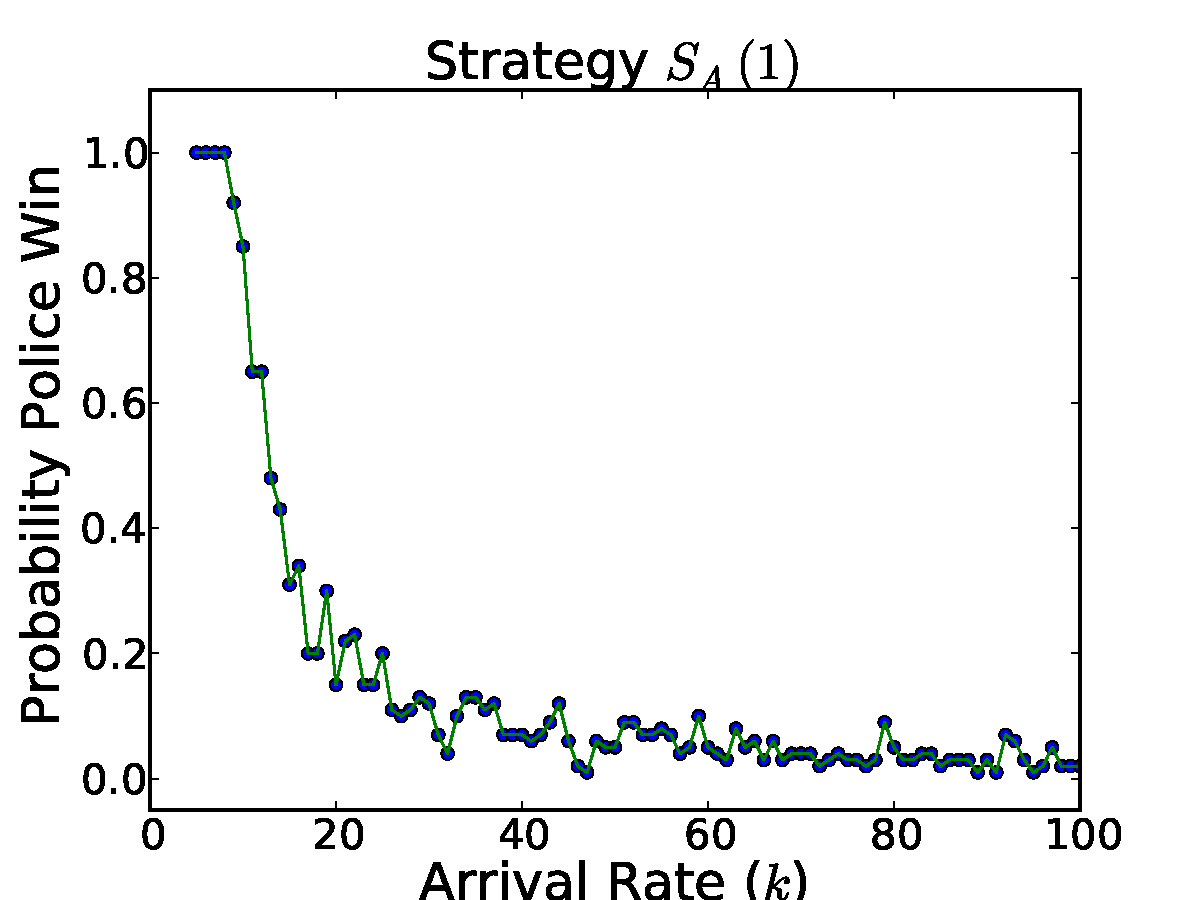
\includegraphics[width=.6\linewidth]{ImprovedPlotS0.pdf}
 \caption{We experimentally determined the probability of winning with strategy $S_A(1)$.  The strategy is successful for $k \leq 8$.  In particular, we estimate Beat$(S_A(1)) \approx 8$.}
 \label{SA(1)}
 \end{figure}
\end{block}

 \end{column}

%-----------------------------------------------------------
%END COLUMN THREE
%-----------------------------------------------------------


\begin{column}{\sepwid}\end{column}			% empty spacer column


%-----------------------------------------------------------
%BEGIN COLUMN FOUR
%-----------------------------------------------------------
\begin{column}{\onecolwid}					  

\begin{block}{Beat($S$)}
Let $S$ be the officers strategy whether to investigate or arrest.  Let:
\begin{align*}
\textrm{Beat}(S) &:=\max\left(k | \substack{\textrm{police eliminate syndicate}\\ \textrm{  in finite time}}\right)
\end{align*}
The greater Beat$(S)$, the more effective a strategy $S$ is against a growing criminal syndicate.  See Figure [\ref{SA(1)}] and [\ref{otherbeats}] for examples.
 \end{block}

 \begin{figure}
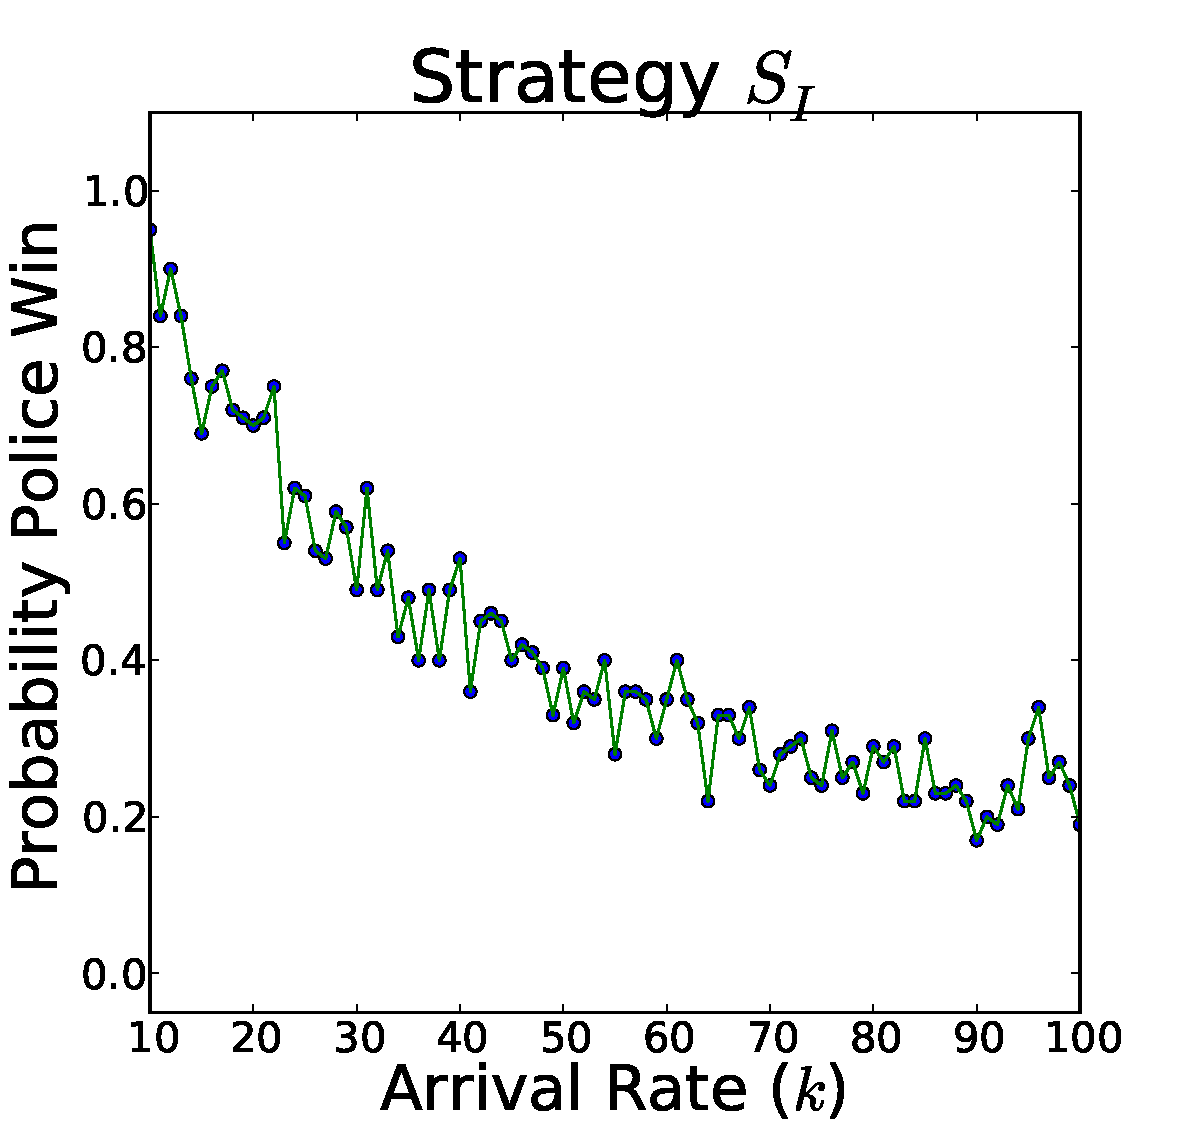
\includegraphics[width=0.5\linewidth]{ImprovedPlotS1.pdf}
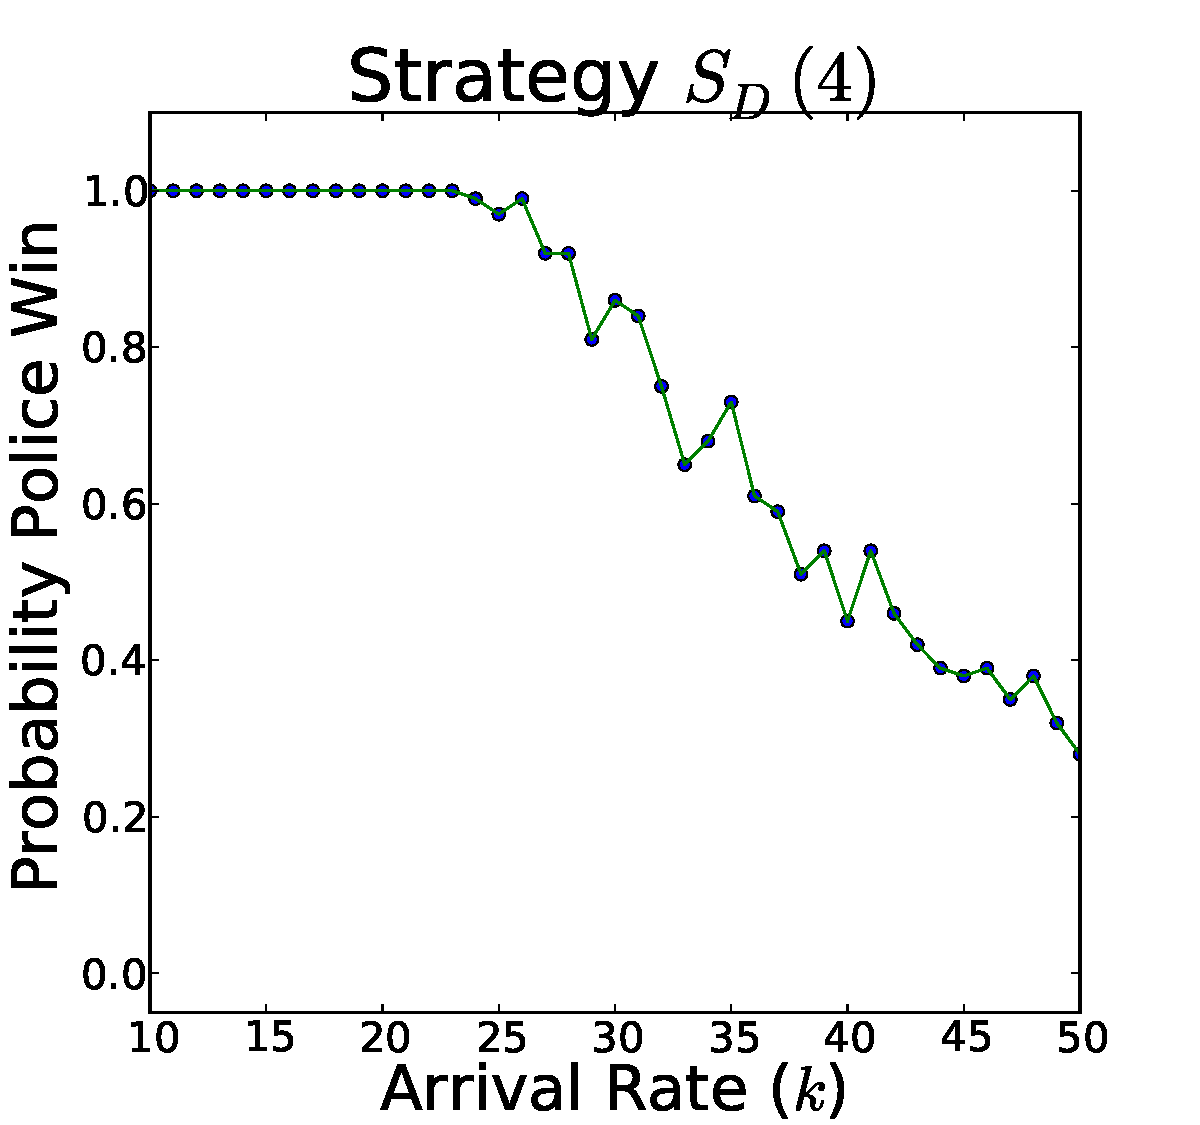
\includegraphics[width=0.5\linewidth]{ImprovedPlotS3.pdf}
 \caption{The probability of winning with $S_D(4)$ and $S_I$.  For $S_I$, there persists a non-zero probability that the root is caught for large $k$.  The right plot suggests Beat$(S_D(4)) \approx 24$.}
 \label{otherbeats}
 \end{figure}
\begin{block}{Conjecture on Pursuit}
For every $p$, there exists a $q$ such that
$$
\textrm{Beat}(S_{D}(q)) > \max(\textrm{Beat}(S_A(p)), \textrm{Beat}(S_I)).
$$
\end{block}

\begin{block}{Acknowledgements}
James von Brecht was instrumental in the early stages of this project.  We used NetworkX, NumPy, and SciPy for all the simulations.  
We used a poster template by Nathaniel Johnston.  
\end{block}
\begin{block}{Bibliography}
\small{\begin{thebibliography}{99}
\bibitem{McCalla} McCalla, Scott G., M. B. Short, and P. J. Brantingham. "The effects of sacred value networks within an evolutionary, adversarial game." Journal of Statistical Physics 151.3-4 (2013): 673-688.
\bibitem{Mahmoud} Smythe, Robert T., and H. Mahmoud. "A survey of recursive trees." Theory of Probability and Mathematical Statistics 51 (1995): 1-28.
%\bibitem{Chayes} Berger, Noam, et al. "Asymptotic behavior and distributional limits of preferential attachment graphs." The Annals of Probability 42.1 (2014): 1-40.
\bibitem{Albert}Albert, R\'{e}ko, and A.L. Barab\'{a}si. "Statistical mechanics of complex networks." Reviews of modern physics 74.1 (2002): 47.
\end{thebibliography}}
\end{block}

\end{column}

\begin{column}{\sepwid}\end{column}			% empty spacer column
%-----------------------------------------------------------
%END COLUMN FOUR
%-----------------------------------------------------------
\end{columns}
\end{frame}
\end{document}
